Il package \textit{gameview} rappresenta la view, responsabile di visualizzare i dati forniti dal model. 
\'E composto da un insieme di scene che estendono FXView che provvede al caricamento di eventuali layout. Inoltre, estendono la trait Scene.

Le scene principali sono:
\begin{itemize}
    \item FXMainScene: rappresenta l'implementazione della scena principale che appare all'utente all'avvio dell'applicazione. Permette di avviare la partita, modificare le impostazioni, guardare i credits o uscire dal gioco.
    \item FXGameScene: rappresenta l'arena di gioco e comprende tutti gli elementi forniti da \textit{gamelogic}. I vari elementi sono rappresentati da case class di supporto a \textit{FXGameScene} ed estendono tutti da una trait GameElements relativa a una serie di elementi generici.
    \item FXSettingsScene: rappresenta le impostazioni, tramite essa si può cambiare il nome del player e la difficoltà del gioco.
    \item FXPlayerRankingScene: rappresenta la classifica del gioco.
    \item FXCreditsScene: rappresenta la i credits.
    
    \begin{figure}[H]
    \centering
      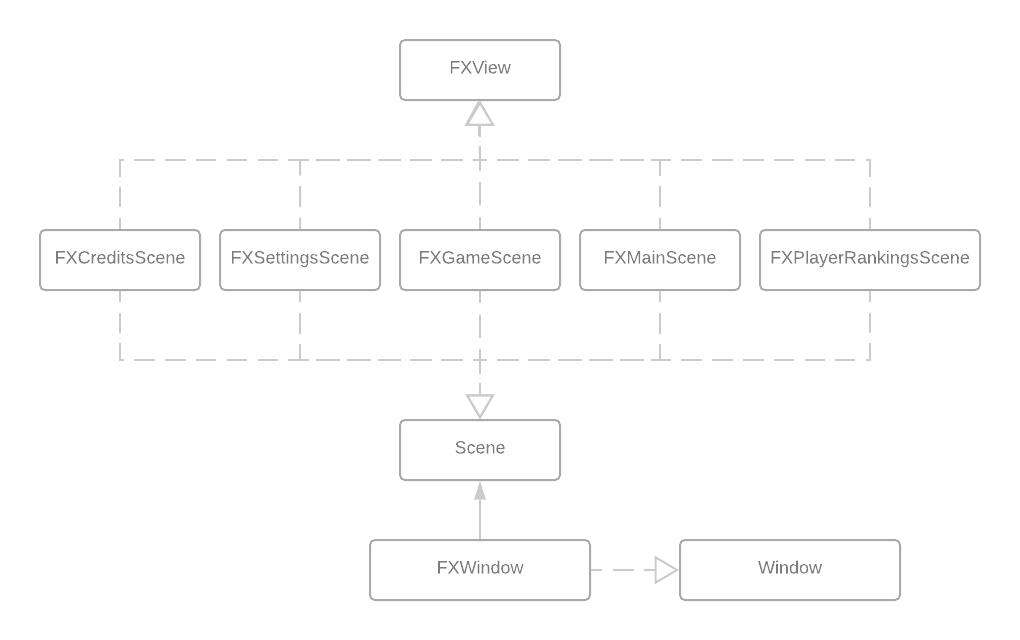
\includegraphics[width=14cm]{res/Scene_Diagram.png}
      \caption{Organizzazione del gameview}
      \label{notifyAction}
    \end{figure}
    
\end{itemize}